\chapter{Posterior Regularization}
Posterior regularization is an alternative way of clustering the phrases.
Unlike a Baysian approach where intuitions about the data are expressed through the priors, posterior regularization imposes constraints on posterior distributions of the data.

In this chapter , we will introduce a basic clustering model with EM 
and look at shortcomings of the basic model. This will motivate us for
more complicated posterior regularized models.
\section{Phrase Clustering Model} 
As a brief recap, the clustering problem we are working with
is to label phrases with $K$ induced categories, where
$K$ is picked manually.
Phrases are obtained from bi-text data.
We also look at context
 words before and after
phrases as cues for clustering.
The relationship between phrases, contexts and categories are
represented with a generative model shown in 
Figure \ref{fig:EM}: a phrase picks a 
category and then that category generates the contex for the phrase.

\begin{figure}[h]
  \centering
  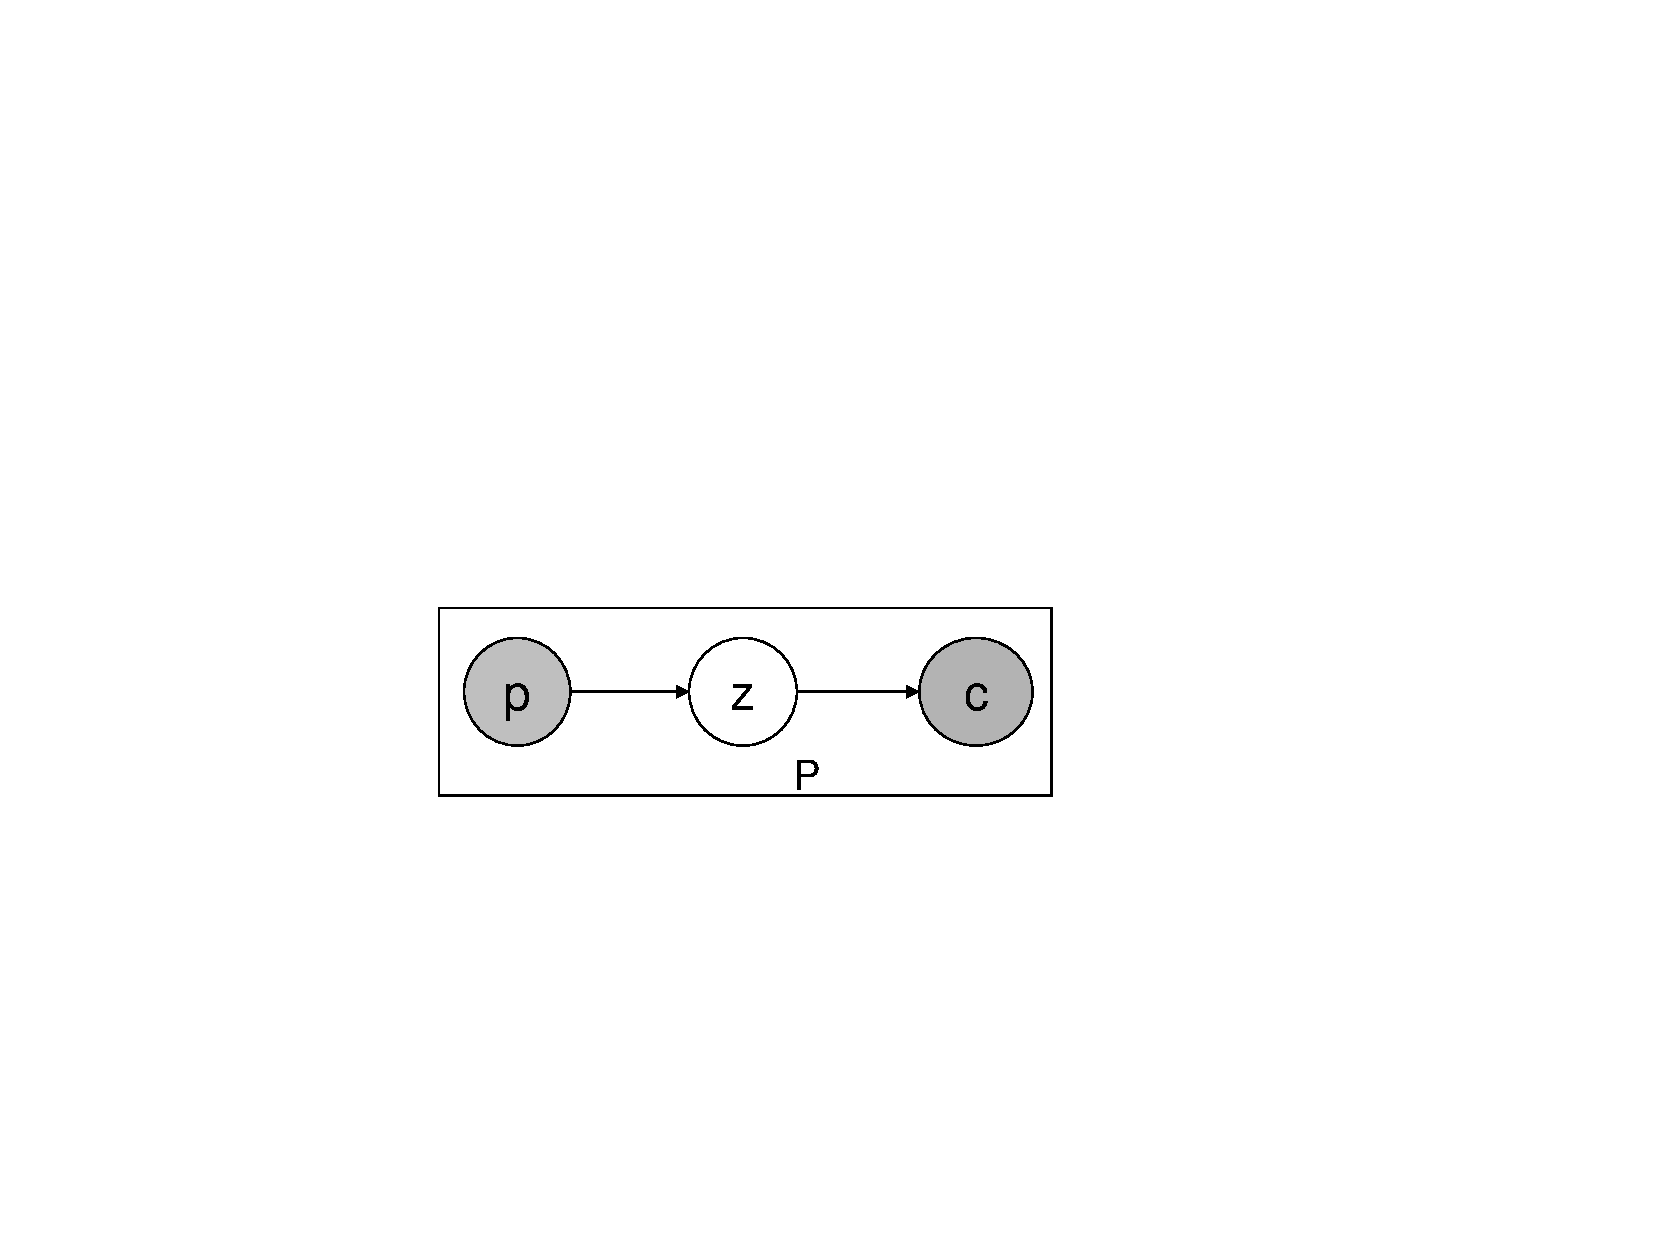
\includegraphics[width=3.5in]{EMdigram}
  \caption{Basic Phrase Clustering Model}
  \label{fig:EM}
\end{figure}

The joint probability of a category $z$ and a context $\bf{c}$ 
given a phrase $\bf{p}$ is
\[
P(z,\bf{c}|\bf{p})=P(z|\bf{p})P(\bf{c}|z).
\]
$P(z|\bf{p})$ is distribution of categories given a phrase.
This can be learned from data.
$P(\bf{c}|z)$ is distribution of context given a category.
Since a context usually contains multiple slots for words, we further
decompose this distribution into independent distributions at
each slot. For example, suppose a context consists of two positions 
before and after the phrase. Denote these words as 
$c_{-2},c_{-1},c_1,c_2$.
Use $P_{-2},P_{-1},P_1,P_2$ to denote distributions of words at each 
position, $P(\bf{c}|z)$ is decomposed as
\[
P(\bf{c}|z)=P_{-2}(c_{-2}|z)P_{-1}
(c_{-1}|z)P_1(c_1|z)P_2(c_2|z).
\]
The posterior probability of a category given a phrase
and a context can be computed by normalizing the joint probability:
\[
P(z|\bf{p},\bf{c})=\frac{P(z,\bf{c}|\bf{p})}
{\sum_{i=1,K}P(i,\bf{c}|\bf{p})}.
\]
With the mechanisms to compute the posterior probabilities, we can 
apply EM to learn all the probabilities.
\section{Sparsity Constraints}
A common linguistic intuition we have about the phrase 
clustering problem is that a phrase should be put into very
few categories, e.g. a verb phrase is unlikely to be used as 
a noun phrase. In other words, the categorization of
a phrase should be sparse.
The generative model we proposed above with EM
allows a phrase to be labelled with many tags. As we observed
from the output, EM is using more categories than we wanted for
each phrase.
Posterior regularization
provides a way to enforce sparsity \citep{ganchev:penn:2009}.
The constraint we use here is called $l_1/ l_\infty$
regularization.